\documentclass[tikz, border=6pt]{standalone}
\usepackage[T1]{fontenc}
\usepackage{lmodern}
\usepackage{amsmath,amssymb,bm}
\usepackage[scaled=0.95]{helvet}
\usetikzlibrary{arrows.meta, positioning}
\definecolor{Blue}{HTML}{3A76D8}
\definecolor{Green}{HTML}{3BA55C}
\definecolor{Orange}{HTML}{EE8133}
\definecolor{Red}{HTML}{DF4B4B}
\definecolor{Gray}{HTML}{6B7280}
\definecolor{Ink}{HTML}{1F2937}
\colorlet{input}{Green}
\colorlet{hidden}{Blue}
\colorlet{output}{Red}
\tikzset{
  block/.style={/utils/exec={\colorlet{pytikzarg}{#1}}, draw=pytikzarg!78!black, fill=pytikzarg!14, rounded corners=3pt, align=center, inner sep=5pt, minimum height=8mm, minimum width=20mm},
  block/.default=Blue,
}
\begin{document}
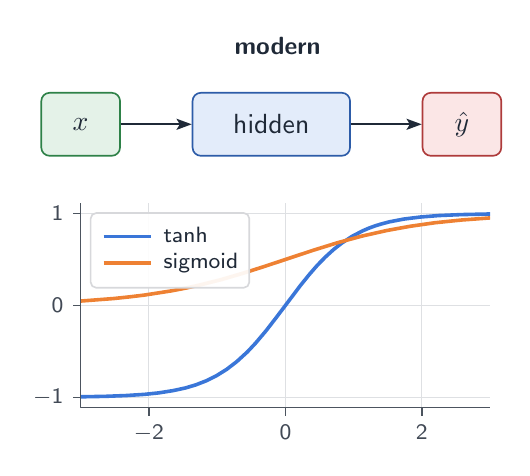
\begin{tikzpicture}[color=Ink, execute at begin picture={\sffamily}, line width=0.6pt, >={Stealth[length=5.5pt, width=4pt, inset=1.2pt]}, line join=round]
  \node[block=input, minimum width=1cm] (n1) at (0,0) {$x$};
  \node[block=hidden, right=0.9cm of n1] (n2) {hidden};
  \node[block=output, minimum width=1cm, right=0.9cm of n2] (n3) {$\hat y$};
  \draw[->] (n1) -- (n2);
  \draw[->] (n2) -- (n3);
  \node[font=\small\bfseries] at (2.5,1) {modern};
  % axes ax1
  \draw[Gray!22, line width=0.4pt] (0.867,-3.6) -- (0.867,-1) (2.6,-3.6) -- (2.6,-1) (4.333,-3.6) --
      (4.333,-1) (0,-3.466) -- (5.2,-3.466) (0,-2.3) -- (5.2,-2.3) (0,-1.134) -- (5.2,-1.134);
  \begin{scope}
    \clip (0,-3.6) rectangle (5.2,-1);
    \draw[color=Blue, line width=1.3pt] (0,-3.461) -- (0.314,-3.455) -- (0.575,-3.445) -- (0.81,-3.43)
        -- (0.993,-3.411) -- (1.176,-3.382) -- (1.333,-3.348) -- (1.463,-3.309) -- (1.594,-3.258) --
        (1.725,-3.193) -- (1.855,-3.112) -- (1.986,-3.011) -- (2.117,-2.891) -- (2.221,-2.78) --
        (2.352,-2.625) -- (2.482,-2.457) -- (2.796,-2.041) -- (2.901,-1.911) -- (3.005,-1.791) --
        (3.11,-1.684) -- (3.214,-1.589) -- (3.319,-1.507) -- (3.449,-1.422) -- (3.58,-1.354) --
        (3.658,-1.32) -- (3.737,-1.291) -- (3.815,-1.267) -- (3.92,-1.239) -- (4.103,-1.204) --
        (4.312,-1.178) -- (4.547,-1.159) -- (4.834,-1.147) -- (5.2,-1.139);
    \draw[color=Orange, line width=1.3pt] (0,-2.245) -- (0.418,-2.213) -- (0.627,-2.191) --
        (0.81,-2.169) -- (1.15,-2.116) -- (1.333,-2.081) -- (1.489,-2.047) -- (1.777,-1.975) --
        (2.064,-1.891) -- (2.326,-1.808) -- (2.953,-1.6) -- (3.266,-1.503) -- (3.58,-1.418) --
        (3.893,-1.348) -- (4.181,-1.296) -- (4.494,-1.251) -- (4.834,-1.216) -- (5.2,-1.189);
  \end{scope}
  \draw[Ink!80, line width=0.5pt] (0,-1) -- (0,-3.6) -- (5.2,-3.6);
  \draw[Ink!80, line width=0.5pt] (0.867,-3.6) -- (0.867,-3.7) (2.6,-3.6) -- (2.6,-3.7) (4.333,-3.6)
      -- (4.333,-3.7) (0,-3.466) -- (-0.1,-3.466) (0,-2.3) -- (-0.1,-2.3) (0,-1.134) -- (-0.1,-1.134);
  \node[anchor=north, font=\footnotesize, text=Ink!85, inner sep=2pt] (ax1-xt0) at (0.867,-3.74) {$-$2};
  \node[anchor=north, font=\footnotesize, text=Ink!85, inner sep=2pt] (ax1-xt1) at (2.6,-3.74) {0};
  \node[anchor=north, font=\footnotesize, text=Ink!85, inner sep=2pt] (ax1-xt2) at (4.333,-3.74) {2};
  \node[anchor=east, font=\footnotesize, text=Ink!85, inner sep=2pt] (ax1-yt0) at (-0.14,-3.466) {$-$1};
  \node[anchor=east, font=\footnotesize, text=Ink!85, inner sep=2pt] (ax1-yt1) at (-0.14,-2.3) {0};
  \node[anchor=east, font=\footnotesize, text=Ink!85, inner sep=2pt] (ax1-yt2) at (-0.14,-1.134) {1};
  \node[anchor=north west, font=\footnotesize, inner sep=4pt, align=left, fill=white, draw=Ink!18, rounded corners=2pt, fill opacity=0.92, text opacity=1] at (0.12,-1.12) {%
    \begin{tabular}{@{}l@{\hspace{4pt}}l@{}}
      \tikz[baseline=-0.6ex]{\draw[color=Blue, line width=1.3pt] (0,0) -- (0.6,0);} & tanh \\
      \tikz[baseline=-0.6ex]{\draw[color=Orange, line width=1.3pt] (0,0) -- (0.6,0);} & sigmoid \\
    \end{tabular}%
  };
\end{tikzpicture}
\end{document}
